\section{$\!\!\!\!\!\!\!$. General Normal Scale Mixture Framework}\label{zyf.four.sec:GeN}    % Section 2

\subsection{Basic properties of $\GeN$ distribution}\label{zyf.four.sec:GeN.definition}        % Section 2.1

Let a positive \trv $\tau$ follow a general continuous distribution with pdf $f_\tau(\tau | \bla)$, where $\bla = (\la_1, \dots, \la_m)$ is an unknown parameter vector. If a \trv $\ibX = (X_1, \dots, X_d)^\top$ has following SR:
\begin{eqnarray}    \label{zyf.four.2.1}
    \ibX \sd \bmu + \frac{\ibZ}{\sqrt{\tau}}, 
\end{eqnarray}
where $\ibZ = (Z_1, \dots, Z_d)^\top \sim N_d(\0, \bSi)$ and $\ibZ \inde \tau$, then $\ibX$ is said to follow the \textit{general mixture of multivariate normal} (Ge-N$_d$) distribution, denoted by $\ibX \sim \GeN$ or $\mbox{Ge-N}_d(\bth)$ with parameter vector $\bth = \{\bmu, \bSi, \bla\}$. In the SR above, we say $\bmu = (\mu_1, \dots, \mu_d) \in \bbR^d$ is the location parameter and $\bSi = (\sigma_{ij})_{d \times d}$ is the scale parameter matrix. Its joint pdf is
\begin{eqnarray}    \label{zyf.four.2.2}
    \mbox{Ge-N}_d(\ibx | \bth) = \frac{1}{(2\pi)^\frac{d}{2} |\bSi|^\frac{1}{2}} \int_0^\infty h_*(\tau | \ibx, \bth) \rd \tau, \quad \ibx \in \bbR^d,
\end{eqnarray}
where $h_*(\tau | \ibx, \bth) = \tau^\frac{d}{2} f_\tau(\tau | \bla) \exp[-\tau(\ibx - \bmu)^\top \bSi^{-1} (\ibx - \bmu) / 2]$. And the conditional distribution of $\tau | \ibX$ is
\begin{eqnarray}    \label{zyf.four.2.3}
    f_{\tau | \ibX} (\tau | \ibx) \pr \tau^\frac{d}{2} f_\tau(\tau | \bla) \exp\left[ -\frac{\tau}{2} (\ibx - \bmu)^\top \bSi^{-1} (\ibx - \bmu) \right], \quad \tau > 0,
\end{eqnarray}
which can be employed to calculate the conditional expectations of $\tau | (\ibX, \bth)$ in the \textit{expectation--maximization} (EM) and \textit{data augmentation} (DA) algorithm in \S\ref{zyf.four.sec:Bayesian}.

Based on SR (\ref{zyf.four.2.1}), we easily obtain the expectation and covariance matrix of $\ibX$ as
\begin{eqnarray}    \label{zyf.four.2.4}
    E(\ibX) = \bmu \qand \Var(\ibX) = E\left( \tau^{-1} \right) \bSi,
\end{eqnarray}
we also consider its kurtosis in each dimension, that is, 
\begin{eqnarray*}
    \Kurt(X_j) = \frac{E\{[X_j - E(X_j)]^4\}}{[\Var(X_j)]^2} - 3 = 3\left\{ \frac{E\left( \tau^{-2} \right)}{\left[ E\left( \tau^{-1} \right)\right]^2} - 1\right\}, \quad j = 1, \dots, d.
\end{eqnarray*}

\begin{remark}{\rm \textbf{(Selection of mixture variable).} In order to completely eliminate the parameter coupling problem between the covariance matrix and the marginal kurtosis and ensure the identifiability, we impose the inverse expectation of mixture variable $E(\tau^{-1}) = 1$ via the scale transformation property in GIGau family (see more details in \S\ref{zyf.four.sec:Specificcase} and \hyperref[zyf.four.sec:SM]{Supplementary Materials}). \hfill$\|$
}\end{remark}

\subsection{MLEs of parameters via N-EM algorithm}\label{zyf.four.sec:NEM}      % Section 2.2

Suppose that $\{\ibX_i\}_{i=1}^n \iid \GeN$ and $\Y{obs} = \{\ibx_i\}_{i=1}^n$ denote the observed data, where $\ibx_i$ is the realizations of $\ibX_i$, the log-likelihood function of $\bth$ is
\begin{eqnarray}    \label{zyf.four.2.5}
    \ell_*(\bth | \Y{obs}) \sr{(\ref{zyf.four.2.2})} -\frac{nd}{2} \log(2\pi) - \frac{n}{2} \log|\bSi| + \sum_{i=1}^n \log \int_0^\infty h_*(\tau | \ibx_i, \bth) \rd \tau,
\end{eqnarray}
Notice that there is a complex integrals in (\ref{zyf.four.2.5}), therefore, some traditional optimization methods like Newton--Raphson algorithm, Fisher scoring algorithm and \textit{minorization--maximization} (MM, \cite{HL2004}) algorithm are not suitable to use. To solve this integrals, we will adopt the N-EM algorithm (\cite{TL2022}) with the following three steps:
\begin{namelist}{01234567}
\item[\hspace*{-0.08cm} \textsf{N-step}:] By normalizing $h_*(\tau | \ibx_i, \bth)$, we construct a \textit{normalizing density function} (ndf)
	$$
       g_*(\tau | \ibx_i, \bth) \teq \frac{h_*(\tau | \ibx_i, \bth)}{\int_0^\infty h_*(s | \ibx_i, \bth) \rd s}, \quad \tau > 0,
	$$
    so that $g_*(\tau | \ibx_i, \btht)$ is also a density function defined on $\bbR_+$, where $\btht$ denotes the $t$-th approximation of the MLE $\hbth$.

\item[\hspace*{-0.08cm} \textsf{E-step}:] To construct a surrogate function satisfying $Q_*(\bth | \btht) \le \ell_*(\bth | \Y{obs})$ and $Q_*(\btht | \btht)$ $=\ell_*(\btht | \Y{obs})$, we use the Jensen's inequality to obtain
	\begin{eqnarray}   \label{zyf.four.2.6}
        Q_*(\bth | \btht) &=& \ct{*} - \frac{n}{2} \log|\bSi| - \frac{1}{2} \sum_{i=1}^n \at{i*} (\ibx_i - \bmu)^\top \bSi^{-1} (\ibx_i - \bmu) \non \\ [2mm]
        && +\; \sum_{i=1}^n \int_0^\infty \log[f_\tau(\tau | \bla)] \cdot g_*(\tau | \ibx_i, \btht) \rd \tau,
	\end{eqnarray}
    which minorizes $\ell_*(\bth | \Y{obs})$ at $\bth = \btht$, where $\ct{*}$ is a constant free from $\bth$ and
    \begin{eqnarray}    \label{zyf.four.2.7}
        \at{i*} \teq \int_0^\infty \tau \cdot g_*(\tau | \ibx_i, \btht) \rd \tau, \quad i = 1, \dots, n.
    \end{eqnarray}
	
\item[\hspace*{-0.08cm} \textsf{M-step}:] Given $\btht$, by maximizing $Q_*(\bth | \btht)$ with respect to $\bth$, we update $\btht$ by
	$$
	   \bthtt = \arg \max_{\bth\in\bTh} Q_*(\bth | \btht).
	$$
\end{namelist}
Given a pre-specified small positive number $\de_0$, the N-, E- and M-steps are alternately repeated until
$$
    \bigg|\frac{\ell_*(\bthtt | \Y{obs}) - \ell_*(\btht | \Y{obs})}{\ell_*(\btht | \Y{obs})}\bigg| \le \de_0,
$$
then we obtain the MLE $\hbth$ of parameter vector $\bth$. Based on (\ref{zyf.four.2.6}), we take the first derivative of $Q_*(\bth | \btht)$ and solve the following system of equations:
\begin{eqnarray*}
    && \frac{\pa Q_*(\bth | \btht)}{\pa \bmu} = \bSi^{-1} \sum_{i=1}^n \at{i*}(\ibx_i - \bmu) = \0_d, \\ [2mm]
    && \frac{\pa Q_*(\bth | \btht)}{\pa \bSi} = -\frac{n}{2} \bSi^{-1} + \frac{1}{2} \sum_{i=1}^n \at{i*}(\ibx_i - \bmu)(\ibx_i - \bmu)^\top \left( \bSi^{-1} \right)^2 = \0_{d \times d}, \\ [2mm]
    && \frac{\pa Q_*(\bth | \btht)}{\pa \la_k} = \sum_{i=1}^n \log \int_0^\infty \frac{\pa \log[f_\tau(\tau|\bla)]}{\pa \la_k} \cdot g_*(\tau | \ibx_i, \btht) \rd \tau = 0, \qfor k = 1, \dots, m.
\end{eqnarray*}
We obtain the $(t+1)$-th approximation of $\hbth$ as
\begin{eqnarray}    \label{zyf.four.2.8}
    \left\{
    \begin{array}{lll}
        \bmutI &=& \dis \frac{\sum_{i=1}^n \at{i*} \ibx_i}{\sum_{i=1}^n \at{i*}} = \bX \ibpt{*}, \\ [6mm]
        \bSitI &=& \dis \frac{1}{n} \sum_{i=1}^n \at{i*} \left( \ibx_i - \bmutI\right) \left( \ibx_i - \bmutI\right)^\top \\ [6mm]
        &=& \dis \frac{1}{n}\left(\bX - \1_n \bmu^{(t+1)\top} \right)^\top \At{*} \left(\bX - \1_n\bmu^{(t+1)\top} \right), \\ [6mm]
        \latI_k &=& \dis \sol\left\{ s_*(\la_k | \Y{obs}, \btht) = 0 \right\}, \qfor k = 1, \dots, m,
    \end{array}
    \right.
\end{eqnarray}
where $\at{i*}$ is defined by (\ref{zyf.four.2.7}), 
$$
    \pt{i*} \teq \frac{\at{i*}}{\sum_{j=1}^n \at{j*}}, \quad i = 1, \dots, n \quad \ibpt{*} \teq (\pt{1*}, \dots, \pt{n*})^\top,  
$$
$\bX = (\ibx_1, \dots, \ibx_n)^\top$, $\At{*} = \diag(\at{1*}, \dots, \at{n*})$ and the symbol ``$\sol\{s_*(\la_k | \Y{obs}, \btht) = 0\}$'' denotes the unique root of the equation $s_*(\la_k | \Y{obs}, \btht) = 0$ with
$$
    s_*(\la_k | \Y{obs}, \btht) = \sum_{i=1}^n \log \int_0^\infty \frac{\pa \log[f_\tau(\tau|\bla^{(t+1,t)})]}{\pa \la_k} \cdot g_*(\tau | \ibx_i, \btht) \rd \tau,
$$
where $\bla^{(t+1,t)} \teq \left( \latI_1, \dots, \latI_{k-1}, \la_k, \lat_{k+1}, \dots, \lat_m \right)^\top$.

\subsection{Mean regression model for $\GeN$ distribution}       % Section 2.3

From (\ref{zyf.four.2.4}), we know the expectation of Ge-N$_d$ distribution is $\bmu$, therefore, by assuming that $\{\ibX_i\} \ind \mbox{Ge-N}_d(\bmu_i, \bSi, \bla)$ and observed data $\Y{obs} = \{\ibx_i, \ibzi\}_{i=1}^n$, we consider the following mean regression model
\begin{eqnarray}    \label{zyf.four.2.9}
    E(\ibX_i | \ibzi) = \bmu_i = \bB^\top \ibzi, \quad i = 1, \dots, n,
\end{eqnarray}
where $\ibzi = (z_{i1}, \dots, z_{iq})^\top$ is a $q$-dimensional vector of covariates for the $i$-th subject, the matrix of regression coefficients
\begin{eqnarray*}
    \bB = \left(
    \begin{array}{cccc}
        \be_{11} & \be_{12} & \cdots & \be_{1d} \\ 
        \be_{21} & \be_{22} & \cdots & \be_{2d} \\ 
        \vdots   & \vdots   & \ddots & \vdots   \\
        \be_{q1} & \be_{q2} & \cdots & \be_{qd}
    \end{array}
    \right),
\end{eqnarray*}
with $q \times d + d(d + 1) / 2 + m \le n$. Let $\bga = \{ \bB, \bSi, \bla\}$ be the parameter vector, based on (\ref{zyf.four.2.2}) and (\ref{zyf.four.2.9}), the log-likelihood function of $\bga$ is
\begin{eqnarray}    \label{zyf.four.2.10}
    \ell(\bga | \Y{obs}) = -\frac{nd}{2} \log(2\pi) - \frac{n}{2} \log|\bSi| + \sum_{i=1}^n \log \int_0^\infty h(\tau | \ibx_i, \ibzi, \bga) \rd \tau,
\end{eqnarray}
where $h(\tau | \ibx_i, \ibzi, \bga) \teq \tau^\frac{d}{2} f_\tau(\tau|\bla) \exp[-\tau(\ibx - \bB^\top \ibzi)^\top \bSi^{-1} (\ibx - \bB^\top \ibzi) / 2]$. To calculate the MLEs of $\bga$, we utilize the N-EM algorithm again. By computing the ndf
$$
    g(\tau | \ibx_i, \ibzi, \bga) \teq \frac{h(\tau | \ibx_i, \ibzi, \bga)}{\int_0^\infty h(s | \ibx_i, \ibzi, \bga) \rd s}, \quad \tau > 0, 
$$
we construct the surrogate function 
\begin{eqnarray*}
    Q(\bga | \bgat) &=& \ct{} - \frac{n}{2} \log|\bSi| - \frac{1}{2} \sum_{i=1}^n \at{i} \left(\ibx_i - \bB^\top \ibzi \right)^\top \bSi^{-1} \left(\ibx_i - \bB^\top \ibzi \right) \\ [2mm]
    && +\; \sum_{i=1}^n \int_0^\infty \log[f_\tau(\tau | \bla)] \cdot g(\tau | \ibx_i, \ibzi, \bgat) \rd \tau,
\end{eqnarray*}
with constant $\ct{}$ and $\at{i} = \int_0^\infty \tau \cdot g(\tau | \ibx_i, \ibzi, \bgat) \rd \tau$ for $i = 1, \dots, n$.

Finally, we maximize $Q(\bga | \bgat)$ respect to $\bga$ in M-step. By solving the following system of equations:
\begin{eqnarray*}
    && \frac{\pa Q(\bga | \bgat)}{\pa \bB} = \sum_{i=1}^n \at{i} \ibzi (\ibx_i - \bB^\top \ibzi)^\top \bSi^{-1} = \0_{q\times d}, \\ [2mm]
    && \frac{\pa Q(\bga | \bgat)}{\pa \bSi} = -\frac{n}{2} \bSi^{-1} + \frac{1}{2} \sum_{i=1}^n \at{i} \left(\ibx_i - \bB^\top \ibzi \right) \left(\ibx_i - \bB^\top \ibzi \right)^\top \left( \bSi^{-1} \right)^2 = \0_{d \times d}, \\ [2mm]
    && \frac{\pa Q(\bga | \bgat)}{\pa \la_k} = \sum_{i=1}^n \log \int_0^\infty \frac{\pa \log[f_\tau(\tau|\bla)]}{\pa \la_k} \cdot g(\tau | \ibx_i, \ibzi, \bgat) \rd \tau = 0, \qfor k = 1, \dots, m.
\end{eqnarray*}
we obtain the $(t+1)$-th approximation of $\hbga$ as
\begin{eqnarray}    \label{zyf.four.2.11}
    \left\{
    \begin{array}{lll}
        \bBtI &=& \dis \left[ \sum_{i=1}^n \at{i} \ibzi \ibziT \right]^{-1} \left[ \sum_{i=1}^n \at{i} \ibzi \ibx_i^\top \right] = \left(\bZ^\top \At{} \bZ\right)^{-1} \left(\bZ^\top \At{} \bX\right), \\ [6mm]
        \bSitI &=& \dis \frac{1}{n} \sum_{i=1}^n \at{i} \left( \ibx_i - \bB^{(t+1)\top} \ibzi\right) \left( \ibx_i - \bB^{(t+1)\top}\ibzi \right)^\top \\ [6mm]
        &=& \dis \frac{1}{n}\left(\bX - \bZ \bBtI \right)^\top \At{} \left(\bX - \bZ \bBtI \right), \\ [6mm]
        \latI_k &=& \dis \sol\left\{ s(\la_k | \Y{obs}, \bgat) = 0 \right\}, \qfor k = 1, \dots, m,
    \end{array}
    \right.
\end{eqnarray}
where $\bZ = (\ibz_{(1)}, \dots, \ibz_{(n)})^\top$, $\At{} = \diag(\at{1}, \dots, \at{n})$, $\bX = (\ibx_1, \dots, \ibx_n)^\top$ and 
$$
    s(\la_k | \Y{obs}, \bgat) = \sum_{i=1}^n \log \int_0^\infty \frac{\pa \log[f_\tau(\tau|\bla^{(t+1,t)})]}{\pa \la_k} \cdot g(\tau | \ibx_i, \ibzi, \bgat) \rd \tau.
$$

\subsection{Bootstrap CIs of $\bth$}     % Section 2.4

The large--sample method for calculating CIs of parameters has two limitations: (1) The asymptotic CI is not reliable for small to moderate sample sizes; and (2) even though for a large sample size, the range of CI may be beyond its bounds when the true value is close to the bounds. To overcome the two difficulties, this subsection presents the bootstrap method (\cite{Efron1992}) to construct the \textit{bootstrap confidence interval} (BCI) (\cite{Hall1988}, \cite{DR1988}) of $\psi \teq u(\bth)$, where $u(\cdot)$ is an arbitrary function of the parameter vector $\bth$ in the $\mbox{Ge-N}_d(\bth)$ distributions.

Based on the observations $\Y{obs} = \{\ibx_i\}_{i=1}^n$, we can first compute the MLEs $\hbth$ of $\bth$ through the N-EM algorithm (\ref{zyf.four.2.8}) or (\ref{zyf.four.2.11}). Then, we generate a bootstrap sample $\{\ibX_i^*= \ibx_i^*\}_{i=1}^n \iid \mbox{Ge-N}_d(\hbth)$ and compute the bootstrap replication $\hpsi^* = u(\hbth^*)$. Independently repeating this process $G$ times, we obtain $G$ bootstrap replications $\{\hpsi^*(g)\}_{g=1}^G$. Hence, a $100(1-\al)$\% BCI of $\psi$ is $[\hpsi_{\rm L}^*, \  \hpsi_{\rm U}^*]$, where $\hpsi_{\rm L}^*$ and $\hpsi_{\rm U}^*$ are the $(\al/2)G$-th and the $(1-\al/2)G$-th order statistics of $\{\hpsi^*(g)\}_{g=1}^G$.

\subsection{Bayesian method}\label{zyf.four.sec:Bayesian}        % Section 2.5

Assume that $\{\ibX_i\}_{i=1}^n \iid \GeN$ and the observed data $\Y{obs} = \{\ibx_i\}_{i=1}^n$. In this section, we perform the empirical Bayesian inference on parameter $\bvth = \{\bmu, \bSi\}$ (\cite{BT1992}). That is, we will compute the posterior mode and generate the posterior sample via ECM algorithm (\cite{MR1993}) and DA algorithm. After generating the posterior sample, the posterior mean, posterior standard error and Bayesian credit interval can be obtained.

In the empirical Bayesian method, our focus is on the parameter $\bvth$, so $\bla$ will be considered as a constant. Therefore, we replace it by $\hbla$, which can be computed by N-EM algorithm in \S\ref{zyf.four.sec:NEM}. Denote the prior distribution of $\bvth$ be $\pi(\bvth)$ and we regard $\Y{mis} = \{\tau_i\}_{i=1}^n \iid f_\tau(\cdot | \hbla)$ as the missing data. Therefore, we obtain the complete data posterior distribution
\begin{eqnarray}    \label{zyf.four.2.12}
    p(\bvth | \Y{com}) \pr L(\bvth | \Y{com}) \cdot \pi(\bvth), \qwi \Y{com} = \{\Y{obs}, \Y{mis}\}.
\end{eqnarray}
Finding the mode of posterior distribution is equivalent to optimizing the function $p(\bvth | \Y{com})$ to obtain the optimized value $\tilde{\bvth}$. We consider the following two situations: the non-information prior and the conjugate prior distribution.

\subsubsection{The ECM algorithm to calculate posterior mode of $\bvth$}        % Section 2.5.1

If we know little about the parameters before experiment, then we need to consider the following non-information (or diffuse) prior distributions:
\begin{eqnarray}    \label{zyf.four.2.13}
    \pi(\bvth) = |\bSi|^{-\frac{d+1}{2}}
\end{eqnarray}
Combine the equations (\ref{zyf.four.2.12}) and (\ref{zyf.four.2.13}), we obtain the posterior distribution
\begin{eqnarray}    \label{zyf.four.2.14}
    p(\bvth | \Y{com}) \pr |\bSi|^{-\frac{n+d+1}{2}} \exp\left[ -\frac{1}{2}\sum_{i=1}^n \tau_i (\ibx_i - \bmu)^\top \bSi^{-1} (\ibx_i - \bmu) \right]
\end{eqnarray}
The CM-step of ECM algorithm is to compute the posterior mode of the complete data, we obtain
\begin{eqnarray*}
    && \tilde{\bmu} = \frac{\sum_{i=1}^n \tau_i \ibx_i}{\sum_{i=1}^n \tau_i} = \frac{\bX^\top \btau}{\1_d^\top \btau} \qand \\ [2mm]
    && \tilde{\bSi} = \frac{\sum_{i=1}^n \tau_i (\ibx_i - \bmu)(\ibx_i - \bmu)^\top}{n + d + 1} = \frac{(\bX - \1_n \bmu^\top)^\top \bT (\bX - \1_n \bmu^\top)}{n + d + 1},
\end{eqnarray*}
where $\bX = (\ibx_1, \dots, \ibx_n)^\top$, $\btau = (\tau_1, \dots, \tau_n)^\top$, $\bT = \diag(\tau_1, \dots, \tau_n)$. Based on (\ref{zyf.four.2.3}), we can compute the conditional expectation of $\tau_i | \ibX_i$. Then the E-step is to replace $\{\tau_i\}_{i=1}^n$ by their conditional expectations
$$
    E(\tau_i | \Y{obs}, \bvth) = \int_0^\infty \tau \cdot g_*(\tau | \ibx_i, \hbla, \bvth) \rd \tau, \quad i = 1, \dots, n.
$$
And according to the posterior distribution (\ref{zyf.four.2.14}), we obtain
\begin{eqnarray}
    && \bmu | (\Y{com}, \bSi) \sim N_d\left( \frac{\bX^\top \btau}{\1_d^\top \btau}, \frac{\bSi}{\1_d^\top \btau} \right) \qand \label{zyf.four.2.15} \\ [2mm]
    && \bSi | (\Y{com}, \bmu) \sim \IWishart_d\left( (\bX - \1_n \bmu^\top)^\top \bT (\bX - \1_n \bmu^\top), n \right), \label{zyf.four.2.16}
\end{eqnarray}
where $\IWishart_d$ means the inverse Wishart distribution (see more details in Appendix \ref{zyf.four.sec:NIW}).

Then we consider the second situation, when the mean and covariance matrices are unknown, the conjugate prior of the multivariate normal distribution is a \textit{normal inverse Wishart} (NIW) distribution (\cite{LW1992}). Therefore, we consider the following conjugate priors:
\begin{eqnarray}    \label{zyf.four.2.17}
    \bmu | \bSi \sim N_d\left( \bmu_0, \frac{\bSi}{\ka_0} \right) \qand \bSi \sim \IWishart_d(\bLa_0, \nu_0),
\end{eqnarray}
where $\nu_0 > d - 1$. That is, $(\bmu, \bSi) \sim \NIW_d(\bmu_0, \ka_0, \bLa_0, \nu_0)$. According to (\ref{zyf.four.2.12}) and (\ref{zyf.four.2.17}), the complete data posterior distribution can be obtained as
\begin{eqnarray}    \label{zyf.four.2.18}
    p(\bvth | \Y{com}) &\pr& |\bSi|^{-\frac{n + \nu_0 + d + 2}{2}} \exp\left[ -\frac{1}{2} \sum_{i=1}^n \tau_i (\ibx_i - \bmu)^\top \bSi^{-1} (\ibx_i - \bmu) \right. \non \\ [2mm]
    && -\; \frac{1}{2}(\bmu - \bmu_0)^\top \bSi^{-1} (\bmu - \bmu_0) - \frac{1}{2}\tr\left(\bLa_0\bSi^{-1}\right)\bigg].
\end{eqnarray}
Therefore, we compute the posterior mode of complete data
\begin{eqnarray*}
    \tilde{\bmu} &=& \frac{\sum_{i=1}^n \tau_i \ibx_i + \ka_0\bmu_0}{\sum_{i=1}^n \tau_i + \ka_0} = \frac{\bX^\top \btau + \ka_0\bmu_0}{\1_d^\top \btau + \ka_0}, \\ [2mm]
    \tilde{\bSi} &=& \frac{\sum_{i=1}^n \tau_i (\ibx_i - \bmu)(\ibx_i - \bmu)^\top + \bLa_0 + \ka_0(\bmu - \bmu_0)(\bmu - \bmu_0)^\top}{n + \nu_0 + d + 2} \\ [2mm]
    &=& \frac{(\bX - \1_n \bmu^\top)^\top \bT (\bX - \1_n \bmu^\top) + \bLa_0 + \ka_0(\bmu - \bmu_0)(\bmu - \bmu_0)^\top}{n + \nu_0 + d + 2},
\end{eqnarray*}
and replace $\{\tau_i\}_{i=1}^n$ by conditional expectations $E(\tau_i | \Y{obs}, \bvth)$. According to the posterior distribution (\ref{zyf.four.2.18}), we obtain
\begin{eqnarray}
    && \bmu | (\Y{com}, \bSi) \sim N_d\left( \frac{\bX^\top \btau + \ka_0\bmu_0}{\1_d^\top \btau + \ka_0}, \frac{\bSi}{\1_d^\top\btau + \ka_0} \right) \qand \label{zyf.four.2.19} \\ [2mm]
    && \bSi | (\Y{com}, \bmu) \sim \IWishart_d(\bf{\Psi}, n + \nu_0 + 1), \label{zyf.four.2.20}
\end{eqnarray}
where the scale matrix $\bf{\Psi} = (\bX - \1_n \bmu^\top)^\top \bT (\bX - \1_n \bmu^\top) + \bLa_0 + \ka_0(\bmu - \bmu_0)(\bmu - \bmu_0)^\top$.

\subsubsection{DA algorithm with an embedded AR algorithm to generate posterior samples}        % Section 2.5.2

In order to make a complete Bayesian inference of $\bvth$, we need to employ the DA algorithm (\cite{TW1987}) to generate sample that follows the posterior distribution. In the I-step of DA algorithm, we need to generate the missing data $\Y{mis} = \{\tau_i\}_{i=1}^n$ from the conditional distribution (\ref{zyf.four.2.3}). Since the function has no explicitly expression, the \textit{acceptance--rejection} (AR) algorithm is used to achieve this step. We choose the envelope density
$$
    m(\tau_i) = \mGamma\left(\tau_i \;\bigg|\; \frac{d}{2} + 1, \frac{(\ibx_i - \bmu)^\top \bSi^{-1} (\ibx_i - \bmu)}{2}\right)
$$
And we compute the ratio
$$
    \frac{f_{\tau_i|\ibx_i}(\tau_i | \ibx_i, \hbla)}{m(\tau_i)} \le f_\tau(\tau_{\rm mod} | \hbla) \cdot \Ga\left(\frac{d}{2} + 1\right) \left[\frac{(\ibx_i - \bmu)^\top \bSi^{-1} (\ibx_i - \bmu)}{2}\right]^{-\frac{d}{2} - 1} \teq C.
$$
Therefore, the step of DA algorithm with an embedded AR algorithm that generates posterior sample is as follows:
\vkL
\IncMargin{0.1em}  % 使得行号不向外突出
\begin{algorithm}[H]  \label{zyf.four.alg1}
    \SetAlgoNoLine % 不要算法中的竖线
    \SetKwInOut{Input}{\textsf{Input}}\SetKwInOut{Output}{\textsf{Output}} % 替换关键词

    \Input{The initial value $\{\bmu^{(0)}, \bSi^{(0)}\}$, MLEs $\hbla$ and the observed data $\Y{obs} = \{\ibx_i\}_{i=1}^n$;}
    \Output{Posterior mean $\Bvth_k$ and Bayesian CI $[\vth_k^{\rm L},\;\vth_k^{\rm U}]$ for $k = 1, \dots, d(d + 3) / 2$.}
    \BlankLine

    \For{ \(t = 1\) {\rm \bf to} \(G\)} {
        \textbf{I-step}: Draw latent variables $\{\tau_i\}_{i=1}^n$ from $f_\tau(\tau_i | \ibx_i, \hbla)$ via AR algorithm;
        
        \quad Step 1: For $i = 1, \dots, n$, construct envelope density
        $$
            m(\tau_i) = \mGamma\left(\tau_i \;\bigg|\; \frac{d}{2} + 1, \frac{(\ibx_i - \bmu)^\top \bSi^{-1} (\ibx_i - \bmu)}{2}\right);
        $$
            
        \quad Step 2: Generate $U_i = u_i \sim U(0, 1)$ and $Y_i = y_i \sim m(\cdot)$ independently;

        \quad Step 3: Set $\tau_i^{(t)} = y_i$ if 
        $$
            u_i \le \frac{f_{\tau_i|\ibx_i}(y_i | \ibx_i, \hbla)}{\Ct{} m(y_i)},
        $$
        \hspace{1.5cm} otherwise, return Step 2.
        
        Repeat Step 2 and 3 on $i = 1, \dots, n$ and obtain missing data $\Y{mis}^{(t)} = \{\tau_i^{(t)}\}_{i=1}^n$.

        \textbf{P-step}: Generate $\bvth = \{\bmu, \bSi\}$ via Gibbs sampler;

        \quad Step 4: Generate $\bmutI \sim \bmu|(\Y{com}^{(t)}, \bSit)$ via (\ref{zyf.four.2.15}) or (\ref{zyf.four.2.19})

        \quad Step 5: Generate $\bSitI \sim \bSi|(\Y{com}^{(t)}, \bmutI)$ via (\ref{zyf.four.2.16}) or (\ref{zyf.four.2.20}).        
    }
    \textbf{Collection of posterior samples:} Abandon the results of the previous $B$ iterations and save the remaining samples $\{\bmut, \bSit\}_{t=B+1}^G$.

    \textbf{Compute the posterior mean:} 
    $$
        \Bvth_k \teq \frac{1}{G-B} \sum_{t=B+1}^G \vth_k^{(t)}, \qfor k = 1, \dots, \frac{d(d + 3)}{2}.
    $$

    \textbf{Compute the Bayesian CI:} $[\vth_k^{\rm L},\; \vth_k^{\rm U}] = [\vth_k^{(\al/2)},\; \vth_k^{(1-\al/2)}]$, $k = 1, \dots, d(d + 3) / 2$, where $\vth_k^{(q)}$ is the $q$-quantile of the posterior sample.
    \caption{\ Posterior mean and Bayesian CI via the DA algorithm}
\end{algorithm}
\DecMargin{0.1em}

\subsection{Four specific cases of $\GeN$ family}\label{zyf.four.sec:Specificcase}       % Section 2.6

In \S\ref{zyf.four.sec:GeN.definition}---\S\ref{zyf.four.sec:Bayesian}, we assume that the mixture variable $\tau$ follows an arbitrary parametric distribution $f_\tau(\tau|\bla)$ and construct $\GeN$ family. Then we will fix $\tau$ as some specific distributions in \textit{generalized inverse Gaussian} (GIGau) family (i.e., gamma, inverse gamma, inverse Gaussian and reciprocal inverse Gaussian) to explore the so-called Ga-N$_d$, IGa-N$_d$, IGau-N$_d$ and RIGau-N$_d$ distributions and study their basic properties, statistical inference together with the corresponding mean regression models (Details are presented in \hyperref[zyf.four.sec:SM]{Supplementary Materials}). This not only expands our alternative distributions for fitting multivariate symmetric continuous data defined on $\bbR^d$, but also brings and extends the existing distributions, such as Students' $t$ and Laplace, as a special cases (i.e., Ga-N$_d$ and IGa-N$_d$) into our Ge-N$_d$ family framework, and gives a unified statistical inference method. Under different parameter combinations, the density function images of three new distributions proposed by us are shown in Figure \ref{zyf.four.fig1}.

\begin{figure}[H]
    \subfigure[$\;$ Ga-N$_d$ distribution;]
    {
        \centering
        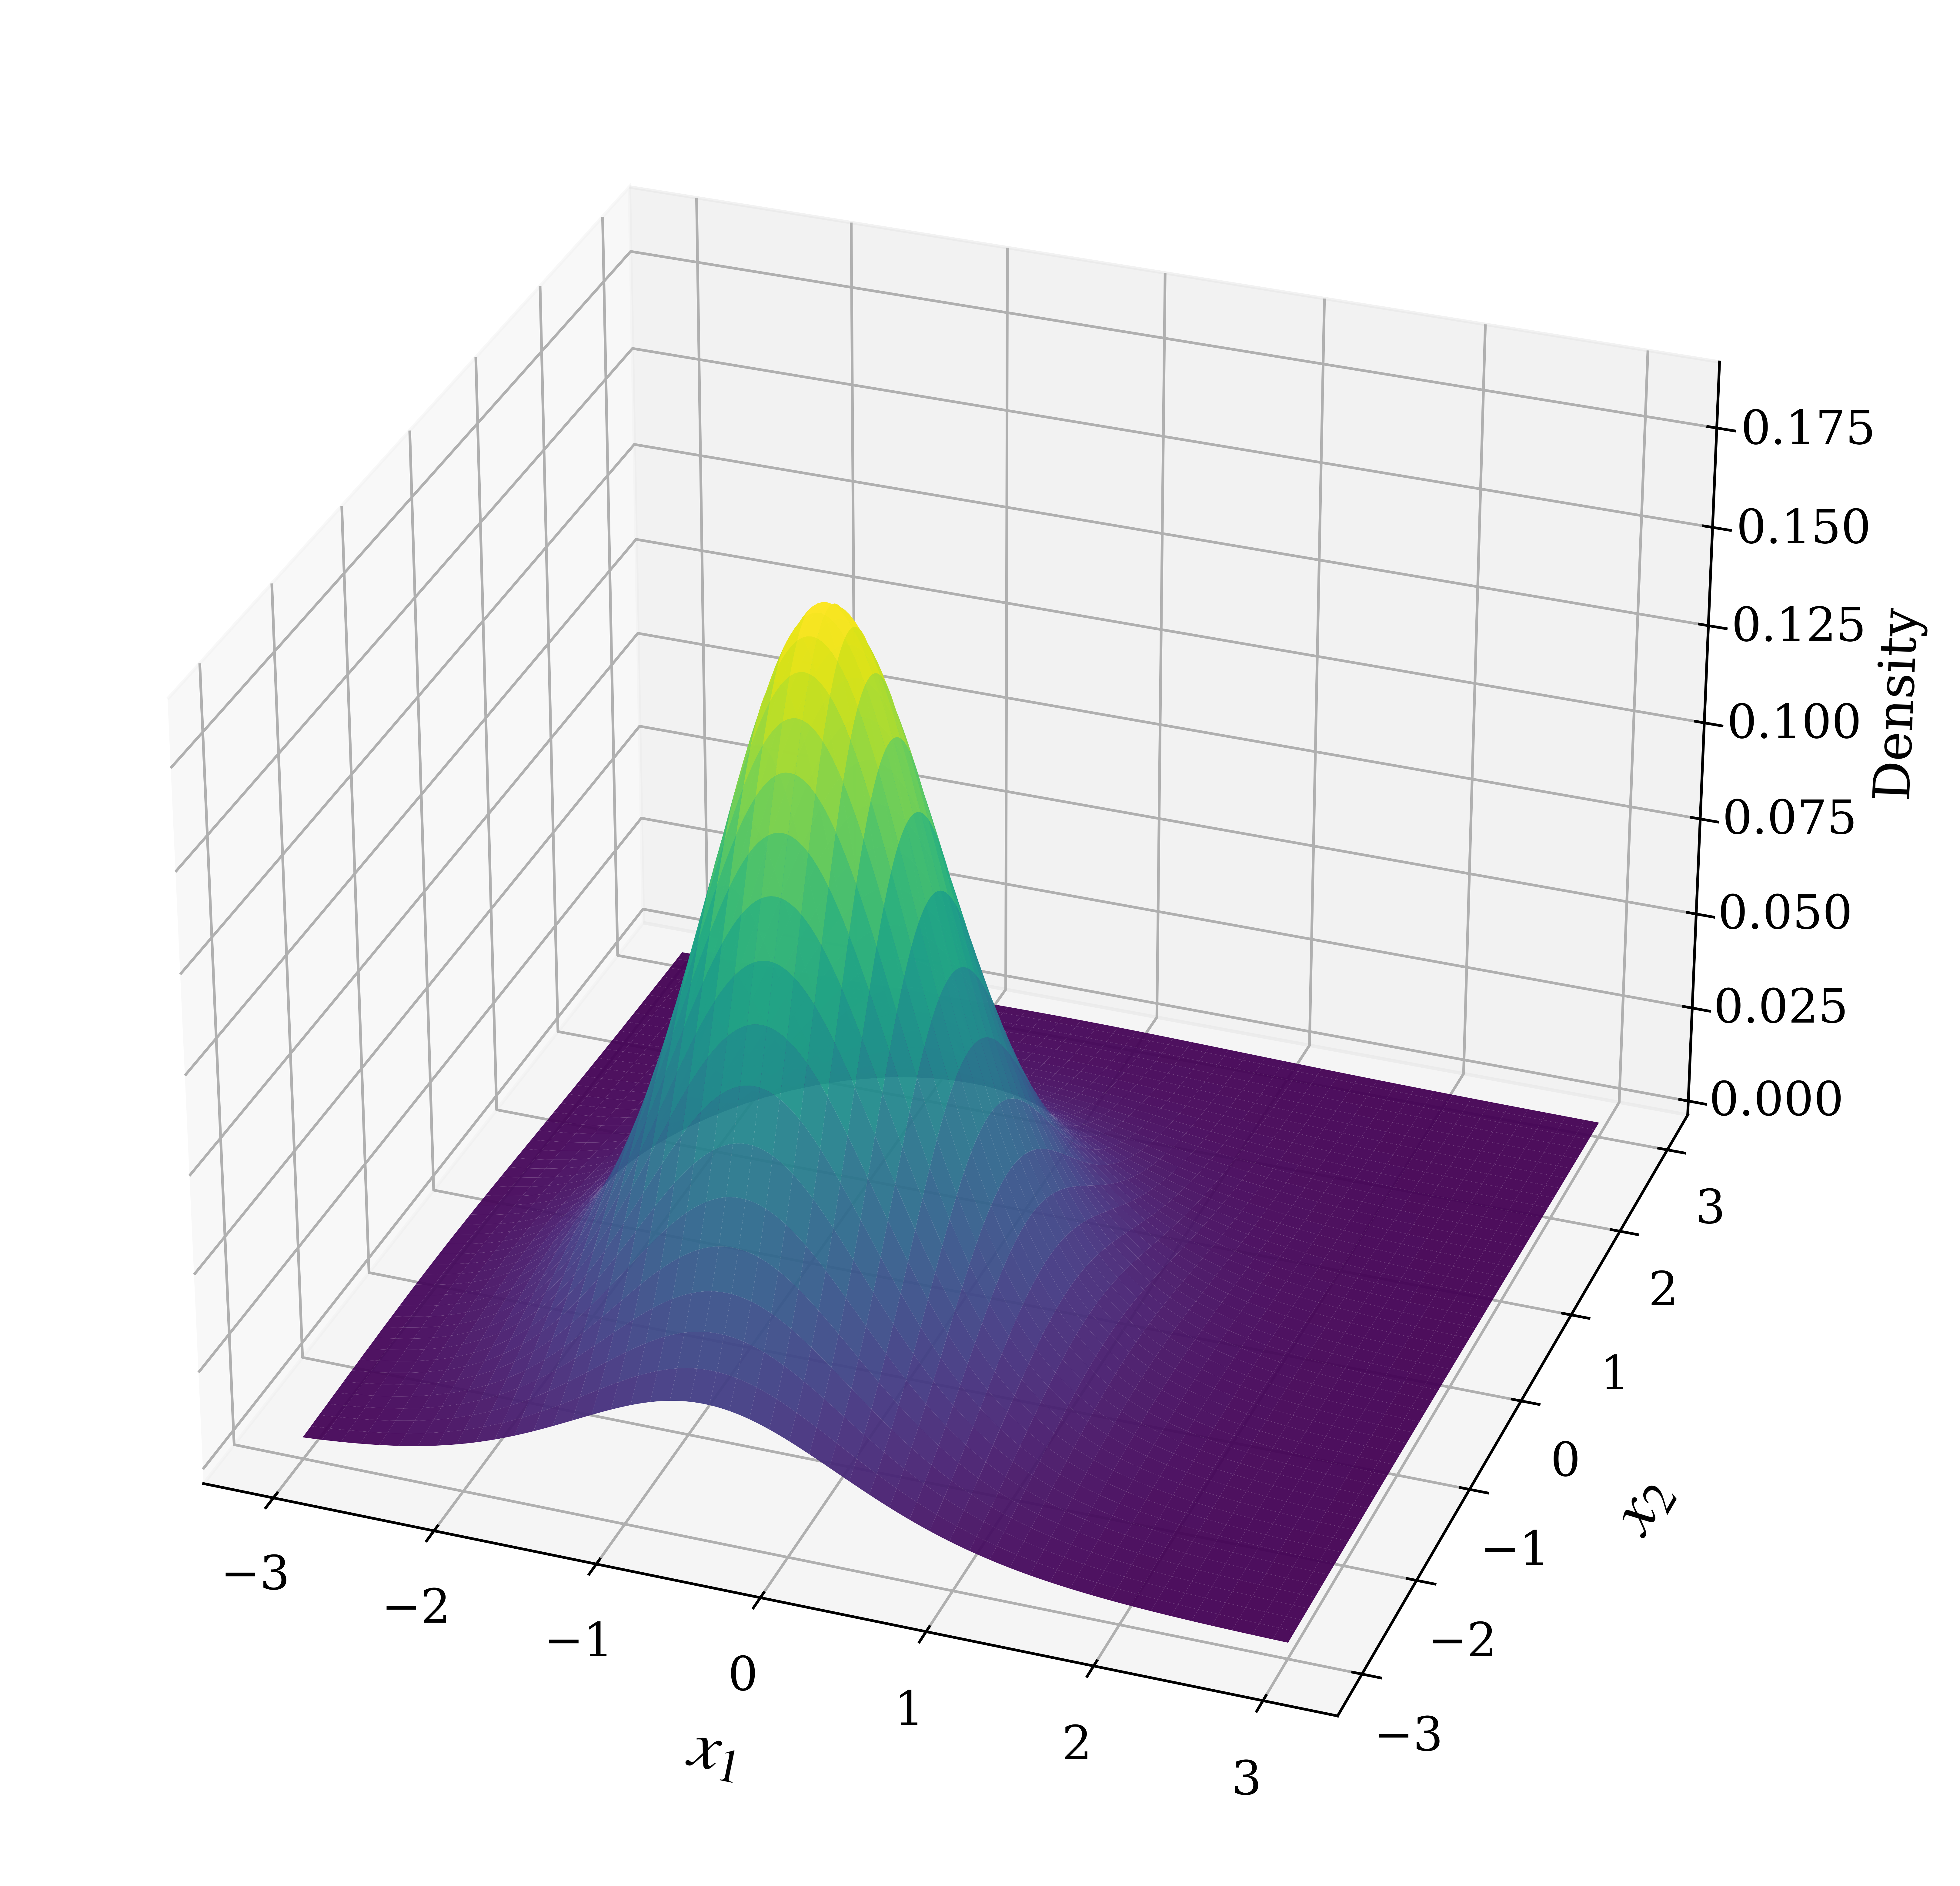
\includegraphics[width=0.5\linewidth]{figures/plot1.png}
    }
    \subfigure[$\;$ IGa-N$_d$ distribution;]
    {
        \centering
        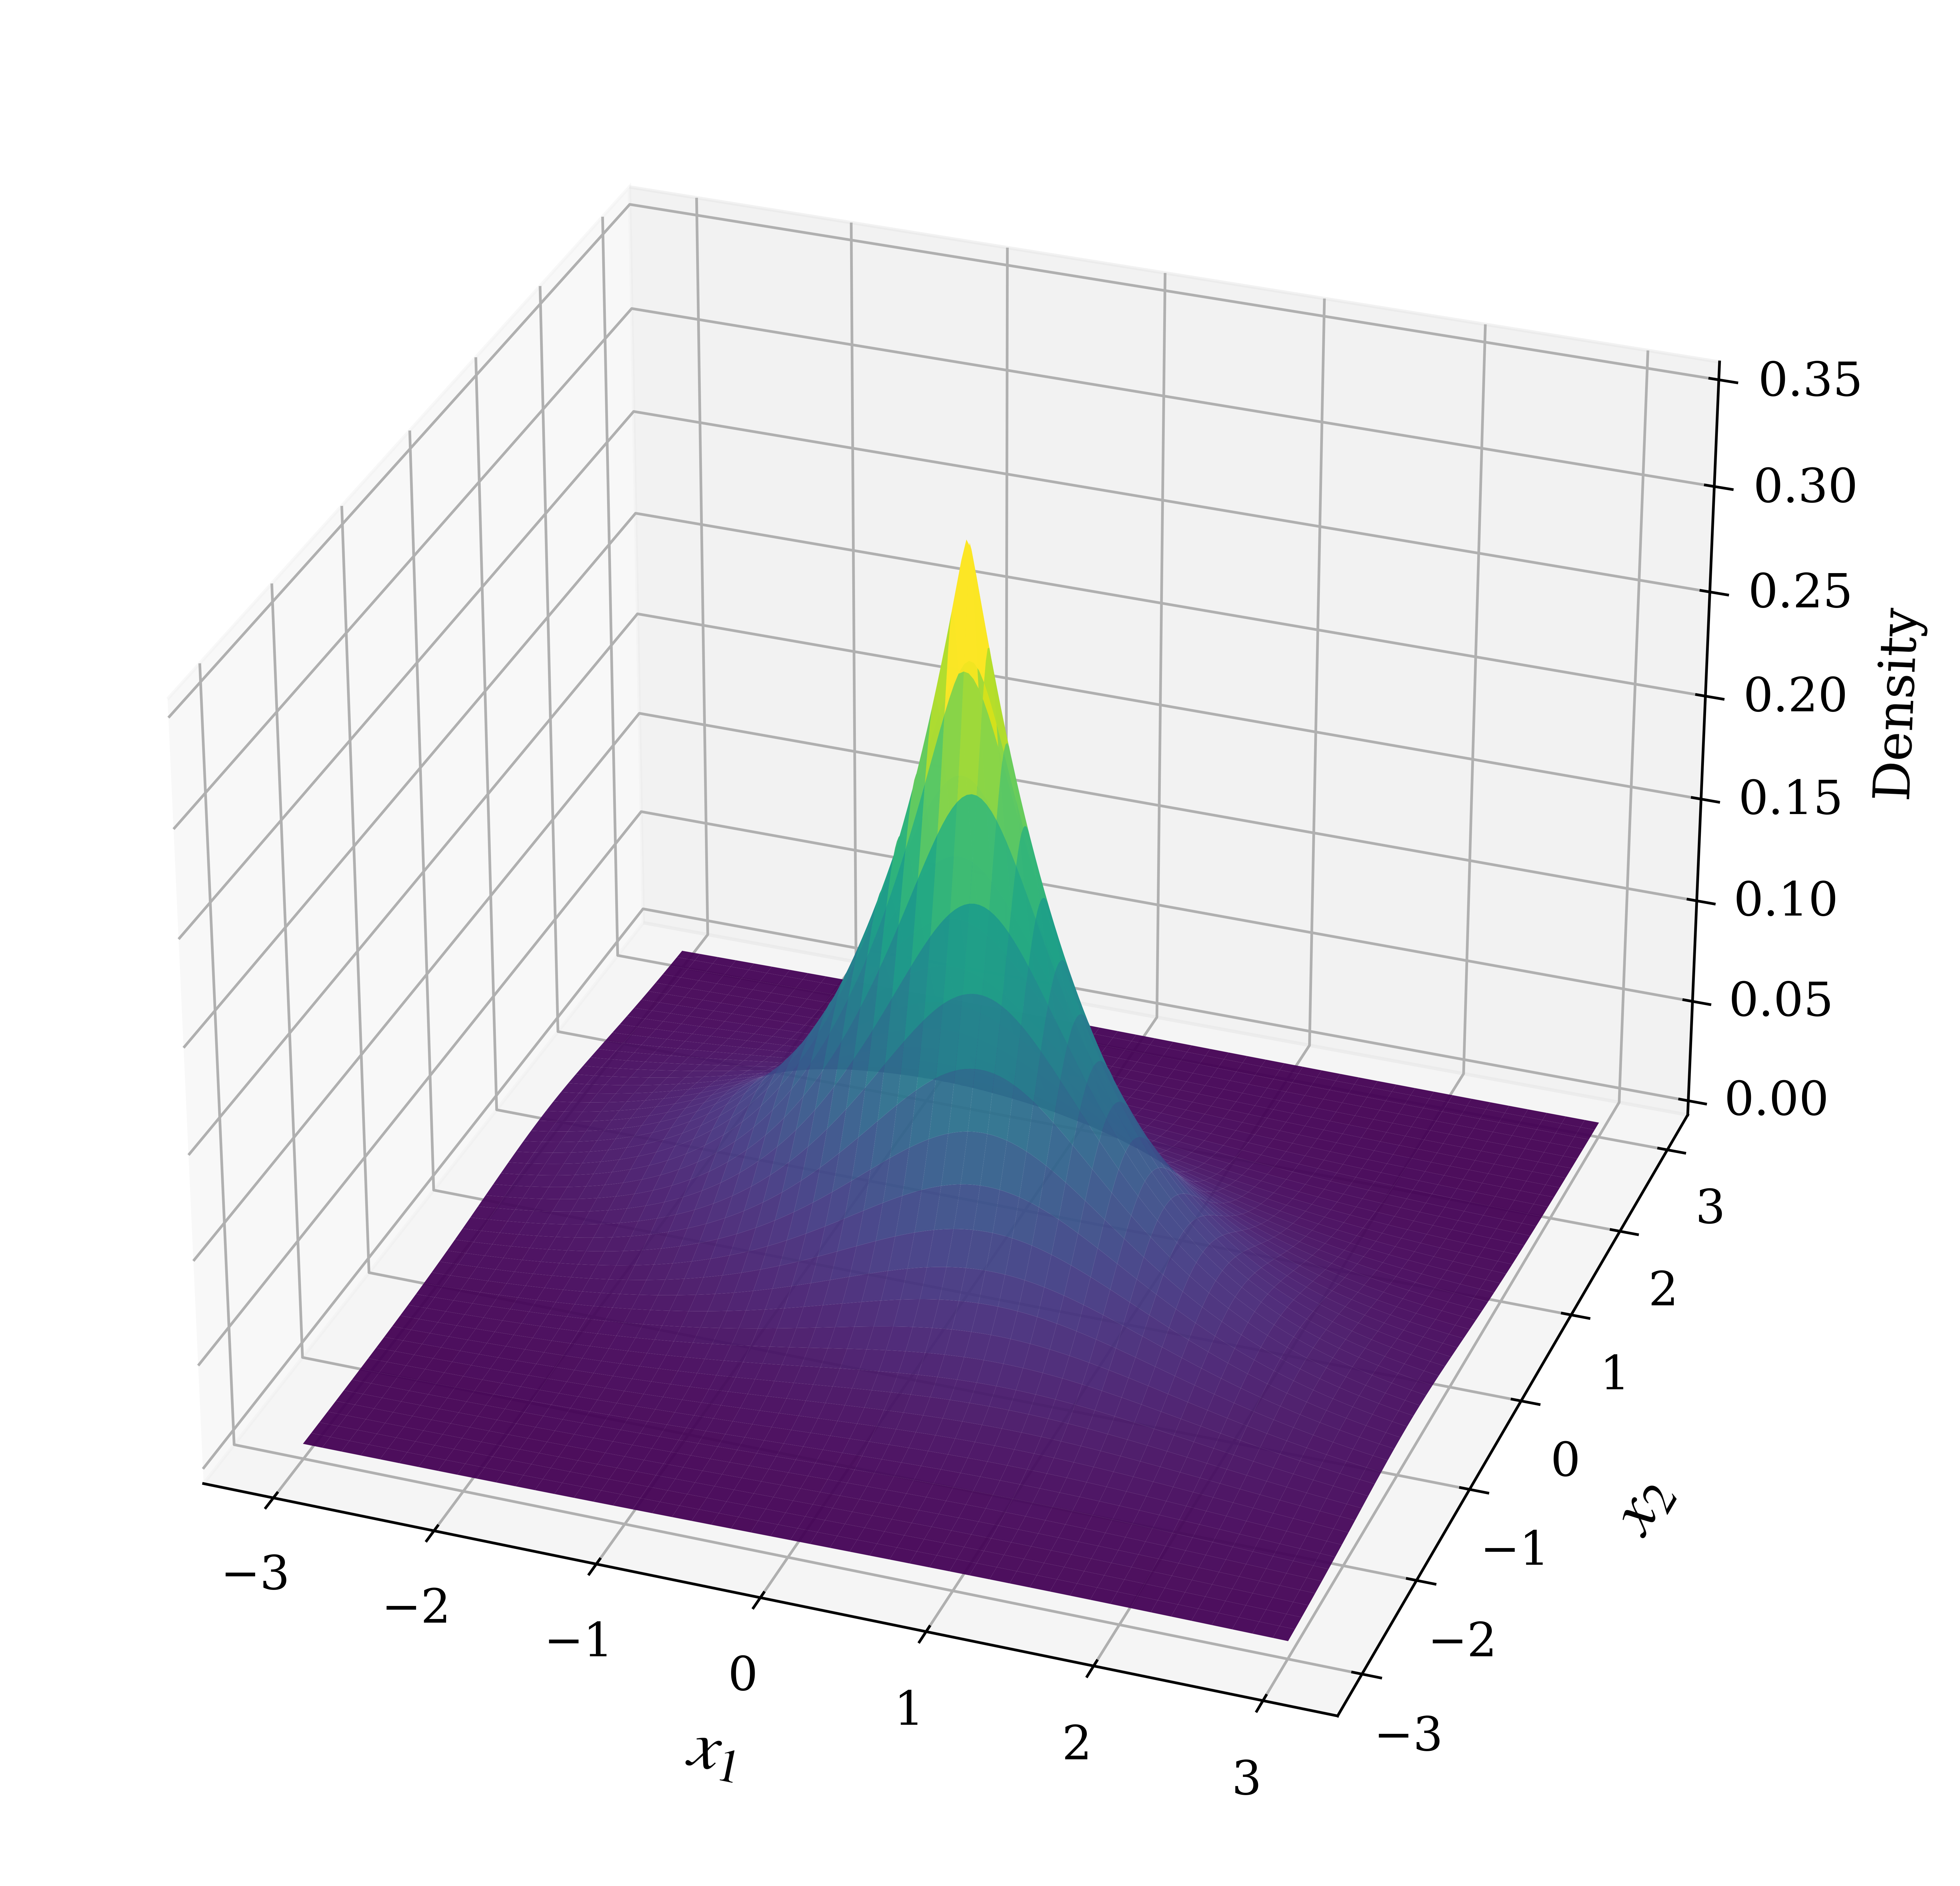
\includegraphics[width=0.5\linewidth]{figures/plot5.png}
    }
    \subfigure[$\;$ IGau-N$_d$ distribution.]
    {
        \centering
        
\includegraphics[width=0.5\linewidth]{figures/plot10.png}
    }
    \subfigure[$\;$ RIGau-N$_d$ distribution.]
    {
        \centering
        
\includegraphics[width=0.5\linewidth]{figures/plot15.png}
    }
    \caption{$\;$ Density of specific cases for Ge-N$_d$ family under various parameter combinations.}
    \label{zyf.four.fig1}
\end{figure}